\subsubsection{一些例子与若干拓扑细节}\label{details}

\begin{figure}
 \begin{center}
     % >>> 原文图 22（原稿第 80 页）
  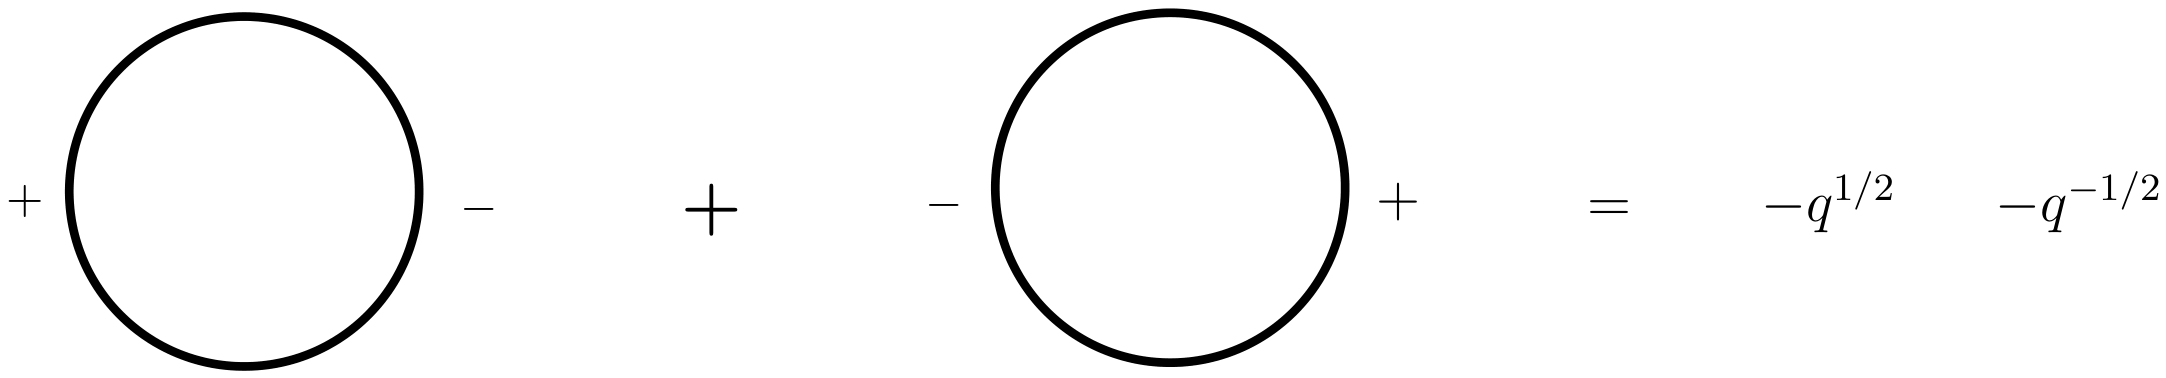
\includegraphics[width=5.5in]{figs/Fig22.png}
 \end{center}
\caption{\small 以最显然的方式投影到平面上的一个平凡纽结。图中没有交叉，但有一个产生事件与一个湮灭事件。在顶点模型中，平凡纽结的不变量通过对纽结两侧（即交叉、产生与湮灭事件之间的各线段）用荷 $+$ 或 $-$ 标记的所有方式进行求和来计算。每个标记以相应局域因子的乘积加权。在当前的例子中，只有图中所示的两种选择给出非零贡献，于是立刻得到结果 $-q^{1/2}-q^{-1/2}$。（原稿第 80 页）}
 \label{unknot}
\end{figure}
作为使用顶点模型的最简单例子，我们来计算一个以显然方式投影到平面上的平凡纽结的期望值（图~\ref{unknot}）。对图形的两种可能标记求和，我们得到结果 $-q^{1/2}-q^{-1/2}$。

\begin{figure}
 \begin{center}
     % >>> 原文图 23（原稿第 81 页）
  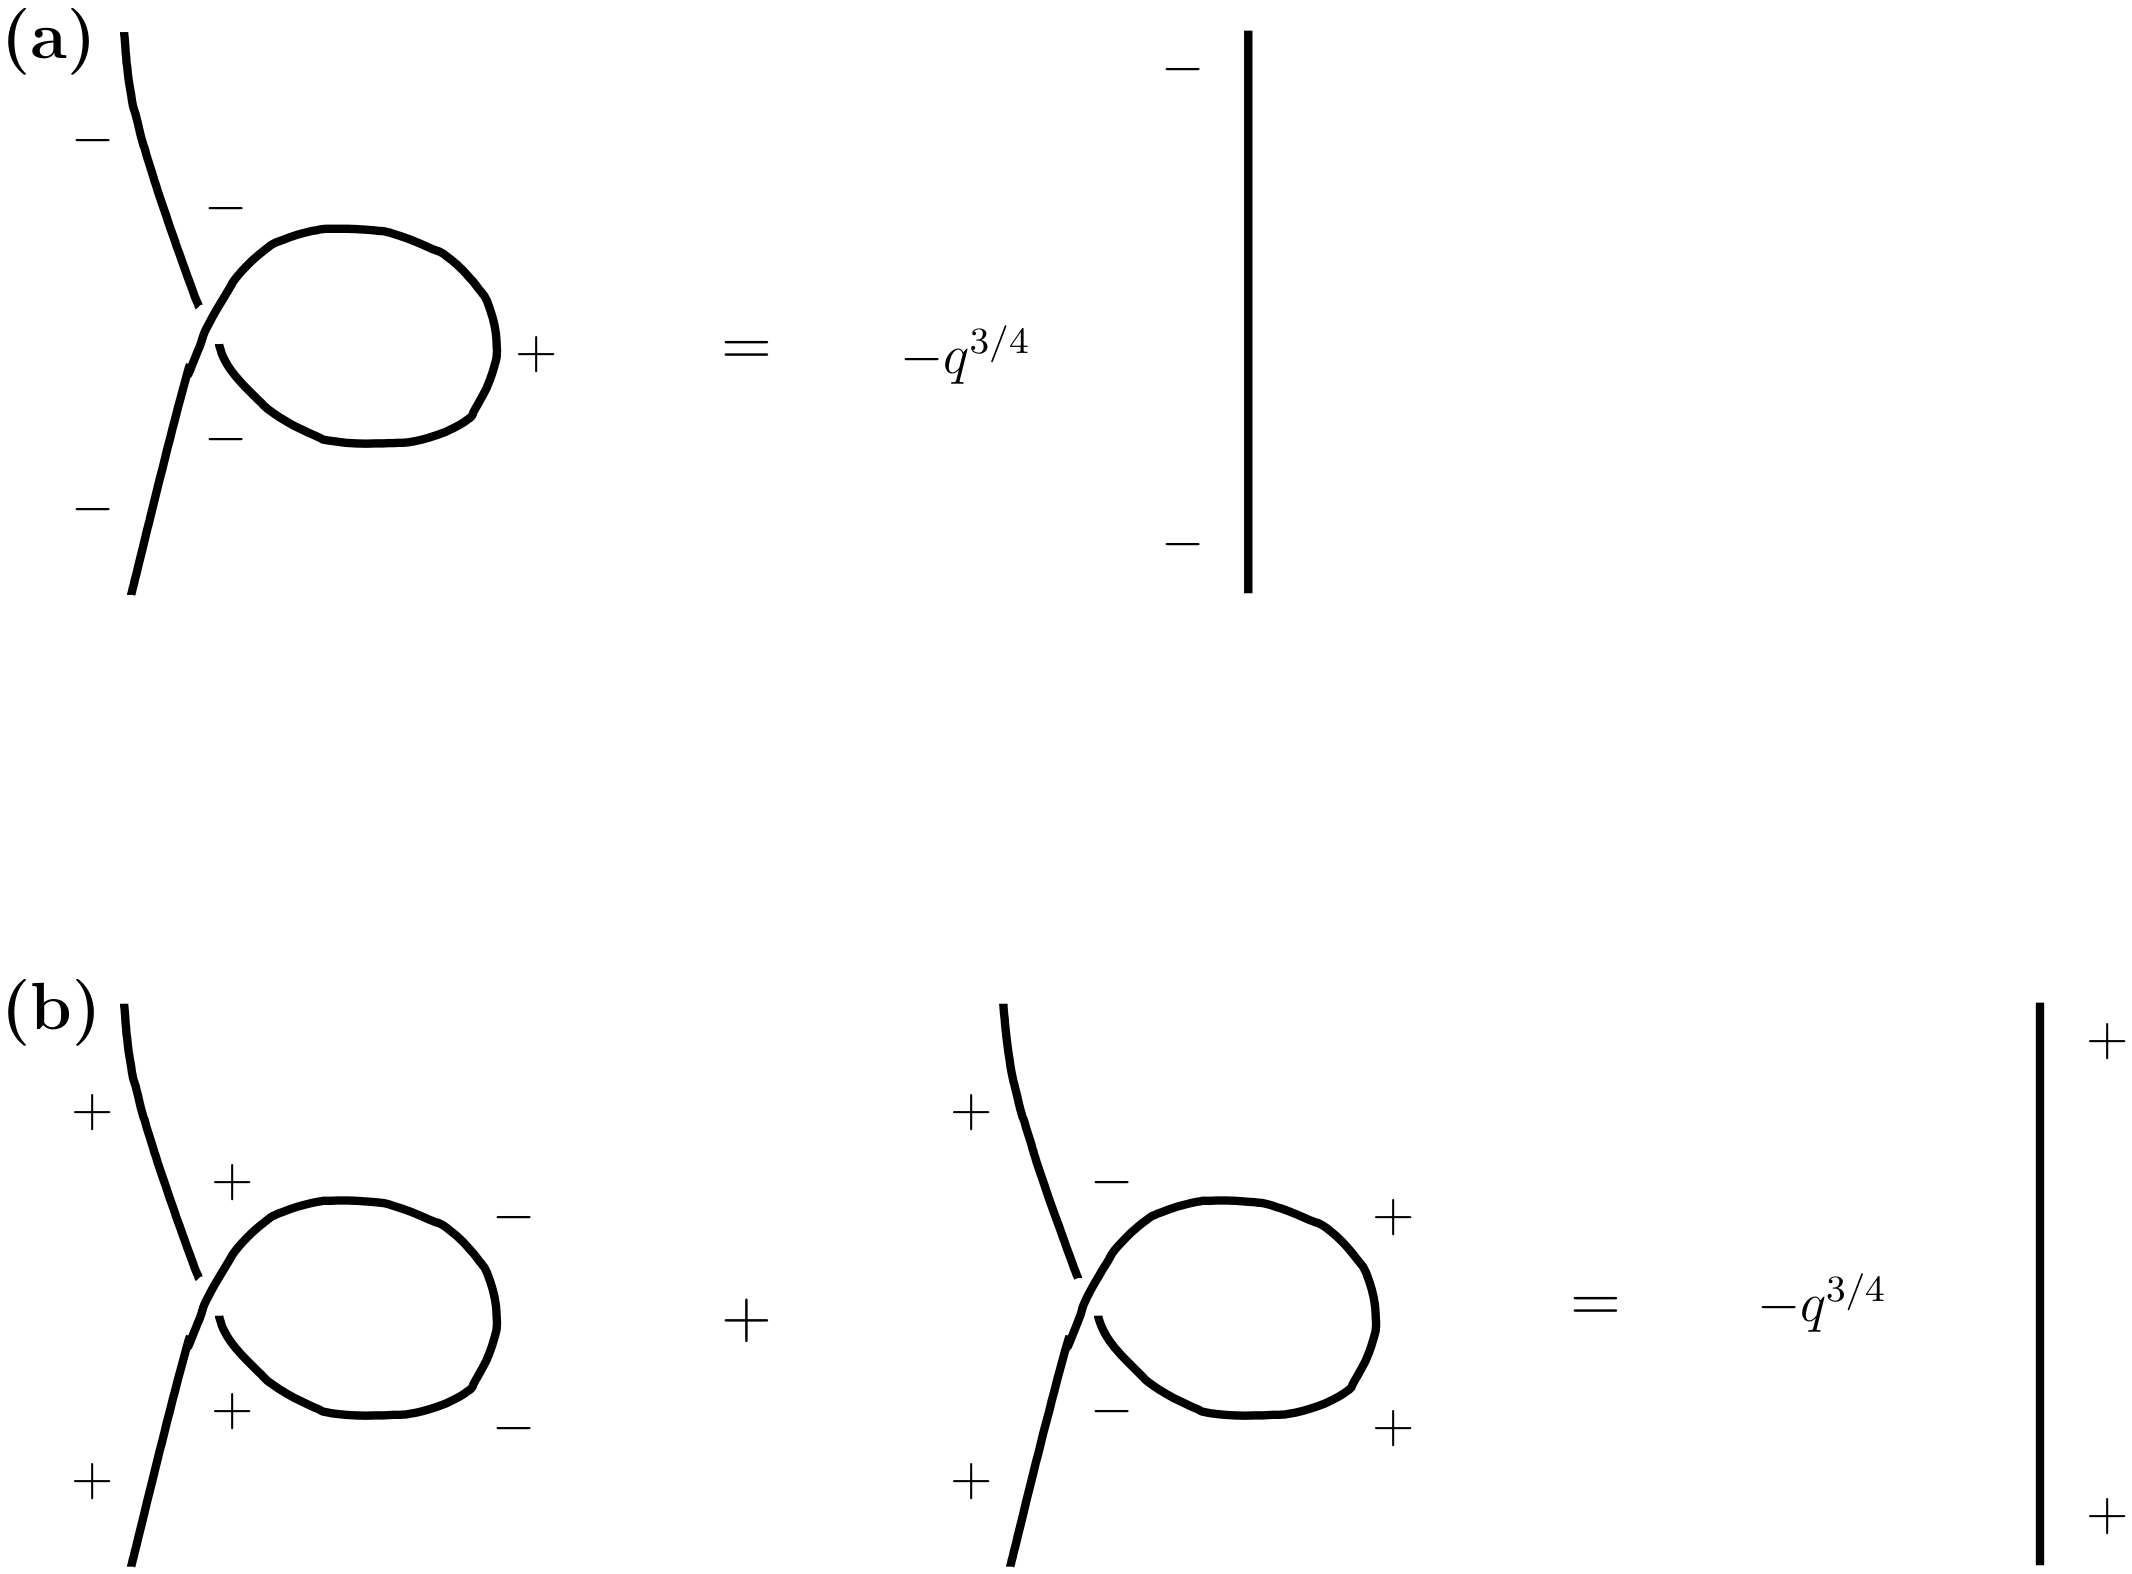
\includegraphics[width=5.5in]{figs/Fig23.png}
 \end{center}
\caption{\small  
 \label{twist}  用顶点模型比较单股到 $x^1-x^3$ 平面的两种不同投影——带扭结（左）与不带扭结（右）。无论该股所带荷的符号如何，扭结都引入一个因子 $-q^{3/4}$。对该股所带荷的两个可能取值，计算相当不同；对荷 $-1$，如 (a) 所示，顶点模型求和只有一个非零贡献，对应于图中标出的标记；但对荷 $+1$，有两种可能的贡献，如 (b) 所示，它们相加得到同一结果。在 (b) 中，第二个贡献涉及一个荷交换过程：上下两股在交叉处交换荷。类似地，若把上穿换成下穿（或把整幅图换成镜像），则相反会给出因子 $-q^{-3/4}$，读者可自行验证。（原稿第 81 页）}
\end{figure}

作为一个稍不那么平凡的例子，我们考虑图~\ref{twist} 所示的单股到 $x^1-x^3$ 平面的两种投影。无论在 (a) 还是 (b) 中，左右两侧所示的纽结投影都可以彼此形变，因此人们也许预期它们等价。
但在当前语境下，事实并非如此。(a) 相对于 (b) 的扭结引入一个因子 $-q^{3/4}$，可以利用顶点模型的权重把它算出来。实际做一遍是有启发性的；无论该股的磁荷是 $+1$ 还是 $ -1$，都出现同一个因子 $-q^{3/4}$，但两种情形下计算的细节相当不同。

% [Tutor Note: 易错点] 这里的关键是“同一个因子、不同的计算”：荷为 $-1$ 时只有一条标记路径非零，因子直接读出；荷为 $+1$ 时有两条路径，其中一条经过荷交换过程，两条贡献相加后才给出同一个 $-q^{3/4}$。若只算其中一条就会得到与荷有关的因子，从而误以为扭结因子不普适。核对时可验证两条贡献的比值恰为 $-q^{-1}$（见 (\ref{twof}) 的相对因子）。

由于因子 $-q^{3/4}$ 不依赖于某一股所带的磁荷，它是普适的：在任意纽结或链环的任意一股上添加图中所示类型的一个扭结，都会使相应的不变量乘以 $-q^{3/4}$。手性相反的类似扭结则使不变量乘以 $-q^{-3/4}$，理由类似。这个因子意味着：量子场论赋予纽结（或链环）的不变量依赖于“标架”（framing）的选取。标架纽结是把纽结稍加增厚成一条带子。人们追踪带子如何扭结，而（在当前语境下）添加一个扭结会使不变量乘以因子 $-q^{3/4}$。以平面投影给出的纽结自带一个自然的标架，它由沿垂直于平面的竖直方向作轻微增厚给出。稍加思考（或用一条纸条做实验）即可看出：尽管在忽略标架时图~\ref{twist}(a) 或 (b) 左右两图在拓扑上等价，它们确实相差一个单位的标架。

% [Tutor Note: 物理图像] 标架（framing）在此不是可有可无的装饰：把纽结增厚成带子后，“扭一下”是拓扑上非平凡的形变，于是不变量只能定义在标架纽结上。本文的顶点模型计算隐含地固定了由“竖直增厚”给出的标架，因此图~\ref{twist} 左右两图虽然作为无标架纽结等价，却相差一个标架单位、恰好给出 $-q^{3/4}$。这也解释了为什么 Jones 多项式需要标架（或等价地，需要把 $q$ 的幂次按 writhe 修正）。

在与二维共形场论相伴的三维纽结不变量的语境下，二维的共形初级场对应于三维中的线算符。若共形初级场的维数为 $h$，那么标架改变一个单位时，相应的线算符要乘以 $\exp(2\pi i h)$。因子 $-q^{3/4}$ 确实就是 $\exp(2\pi i h)$，其中退化 Virasoro 初级场 $V_{-k/2b}$ 的共形维数为
\begin{equation}\label{maxi} h_V(k) =-\frac{k}{2}-\frac{k(k+2)}{4b^2},\end{equation}
此外 $q=\exp(-2\pi i/b^2)$，而我们描述的顶点权重是针对最小荷情形 $k=1$ 的。

% [Tutor Note: 易错点] 请核对这个恒等式：把 $k=1$ 代入 (\ref{maxi}) 得 $h_V(1)=-\frac12-\frac{3}{4b^2}$，故 $\exp(2\pi i h_V(1))=e^{-\pi i}\cdot e^{-3\pi i/(2b^2)}=-q^{3/4}$（其中用到 $q^{3/4}=e^{-3\pi i/(2b^2)}$）。负号来自 $e^{-\pi i}$，即 $k/2$ 这一项；若漏掉它，就会得到 $+q^{3/4}$，与顶点模型的计算不符。这也正是下一段 Chern-Simons 归一化差异的来源。

至此出现一个重要细节。我们所描述的顶点权重适用于 Jones 多项式的某种自然归一化，这种归一化在文献中（例如文献~\cite{Kauffman} 中）被使用。然而，在 $SU(2)$ Chern-Simons 理论中出现的是略有不同的归一化。在 Chern-Simons 理论中，由 $SU(2)$ 二维表示标记的平凡纽结的期望值为 $q^{1/2}+q^{-1/2}$，其符号与我们用顶点权重在图~\ref{unknot} 中得到的相反。（这个符号在 Chern-Simons 理论中容易核对。由于在 $SU(2)$ Chern-Simons 理论中 $q=\exp(2\pi i/(\k^\vee+2))$，其中 $\k^\vee$ 是能级，弱耦合极限 $\k^\vee\to\infty$ 对应于 $q=1$；当 $q=1$ 时，任一表示中 Wilson 圈的期望值就是该表示的维数，对二维表示而言为 $+2$。）类似地，与 $SU(2)$ 自旋 $j=k/2$ 的表示相关的初级场的维数为
\begin{equation}h_{\mathrm{CS}} (k)=\frac{k(k+2)}{4(\k^\vee+2)},\end{equation}
于是在标架改变一个单位时获得的因子为 $\exp(2\pi ih_{\mathrm{CS}})=q^{3/4}$，不带图~\ref{twist} 中出现的负号。显然，符号的差异反映了如下事实：$h_V(k)-h_{\mathrm{CS}}(k)=-k/2$，它与 $b$ 和 $\k^\vee$ 无关。

与 Chern-Simons 理论的比较对本论文未必构成问题，因为我们只是从四维规范场论方程 (\ref{bpseqns}) 出发。然而，人们希望知道，在文献~\cite{fiveknots} 所给出的 Chern-Simons 理论 Wilson 算符与边界奇异磁单极子之间的对偶的语境下，这些符号的最佳解释是什么。我们相信，解释或许是：Chern-Simons 理论中自旋 $k/2$ 的 Wilson 算符，其对偶实际上是边界上的一个 't Hooft 算符，它带有角动量 $k/2$，并在 $k$ 为奇数时是费米性的。（对于定义在四维流形边界上的 't Hooft 算符，相关的旋转群是 $SO(2)$，或更确切地说是其双重覆盖 $\mathrm{Spin}(2)$；该群是阿贝尔的，具有一维表示，以角动量 $k/2$ 标记。）
奇数 $k$ 的费米统计会为每个交叉给出一个负号（相对于图~\ref{vertexweights} 所呈现的内容），并为每个闭合圈给出一个负号；把这些符号计入后，由 Virasoro 退化场编织得到的结果就与在 Chern-Simons 理论中编织得到的结果一致。

最后，把图~\ref{twist} 中的计算与规范群简单取为 $G=U(1)$（而非 $SO(3)$）时的相应计算作比较，是有启发性的。会有两处差别。第一，图~\ref{creation} 中与一对股的产生和湮灭相伴的因子将简单地等于 1。（那些因子完全来自在低能下约化为有效阿贝尔描述时对 $SO(3)$ 理论大质量自由度的积分掉。）第二，对 $G=U(1)$，荷交换过程不存在（因为没有光滑磁单极子），因此图~\ref{twist}(b) 中的第二个贡献将不存在。回顾图~\ref{vertexweights} 可见，对 $G=U(1)$，图~\ref{twist}(a) 或 (b) 的计算给出简单的因子 $q^{1/4}$，而不是 $-q^{3/4}$。
有两点评论：\begin{itemize}\item 对 $G=U(1)$，图~\ref{twist} 的负号不存在（类似地，图~\ref{unknot} 中的负号也不存在）。\item 在 Chern-Simons 理论中，$q$ 的幂次是 $G^\vee$ 相应表示的二次 Casimir 不变量。最高权为 $j$ 的表示的二次 Casimir，对 $G^\vee=U(1)$ 为 $j^2$，对 $G^\vee=SU(2)$ 为 $j(j+1)$。对 $j=1/2$，这在阿贝尔与非阿贝尔情形下分别给出 $q^{1/4}$ 与 $q^{3/4}$。\end{itemize}

% [Tutor Note: 数学工具] 二次 Casimir 的比较给出了一个方便的记账规则：$q$ 的幂次 $=$ 表示的最高权 $j$ 的函数，$U(1)$ 用 $j^2$、$SU(2)$ 用 $j(j+1)$。对 $j=1/2$ 分别得 $1/4$ 与 $3/4$，正好解释图上看到的 $q^{1/4}$ 与 $q^{3/4}$；这也说明为什么非阿贝尔情形会出现“多出来”的 $j$ 项（即 $j(j+1)-j^2=j$）。核对任何顶点权重时，先数出表示的最高权，再套此规则，可迅速判断指数是否算对。

\subsubsection{梯度流与弦}\label{morsestrings}

\begin{figure}
 \begin{center}
     % >>> 原文图 24（原稿第 83 页）
  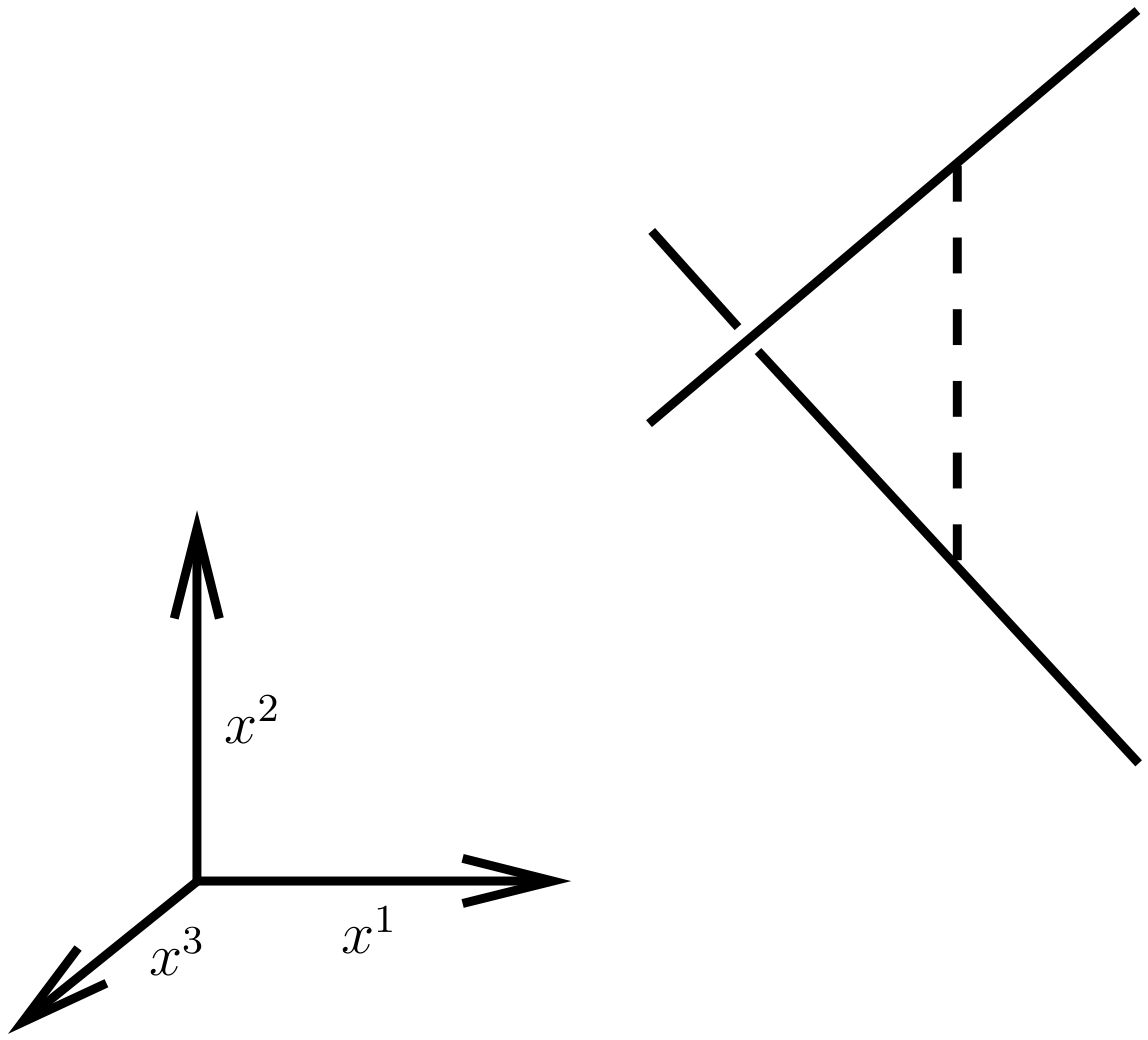
\includegraphics[width=3in]{figs/Fig24.png}
 \end{center}
\caption{\small 为使荷交换过程更清楚可见，我们相对于图~\ref{crossing} 交换了坐标轴。$x^2$ 轴现在竖直，而 $x^1$ 水平。荷交换发生在这样的 $x^1$ 值处：两股在该处仅在 $x^2$ 的取值上不同；因此按本图的坐标轴取向，荷交换涉及沿竖直方向的荷流动，由虚线表示。我们把它解释为 BPS 孤子的传播。该孤子沿对称性破缺轴传播，因此它由仅含实对称性破缺的解来描述——实际上就是由式 (\ref{onl}) 的裸 Miura oper 描述，不含 't Hooft 算符且只有一个 Bethe 根。（原稿第 83 页）\label{soliton}}
\end{figure}
我们可以对适当荷的股交叉时出现的梯度流给出更具体的物理解释。磁荷从一股传播到另一股，可以用一个磁单极子在这两股之间的运动来描述。
若旋转坐标并把 $x^2$ 方向视为“时间”，我们就应当能把相关对象看成仅存在实对称性破缺时的不含时解。

事实上，我们已经精确描述过所需的解：它对应于式 (\ref{onl}) 所描述的、只有一个 Bethe 根且没有奇异磁单极子的裸 Miura oper。因此我们把荷交换过程形象化为一个物体沿 $x^2$ 方向的传播，如图~\ref{soliton} 所示。这一图像过于简化，因为它忽略了垂直于包含纽结的边界 $\R^3$ 的第四维的存在。展示 $y$ 方向作用的另一种图像见图~\ref{bending}。沿 $x^2$ 方向传播时，孤子会停在由裸 Miura oper 的解所给出的某个 $y$ 值处。（如何计算这个值，在第~\ref{supermon}~节有最完整的说明。）当然，这一描述只有在孤子在 $x^2$ 方向传播得足够远、从而有“时间”达到 $y$ 的平衡值时才成立。因此它只在各股彼此充分远离、或对称性破缺足够强时才成立。
\begin{figure}
 \begin{center}
     % >>> 原文图 25（原稿第 84 页）
  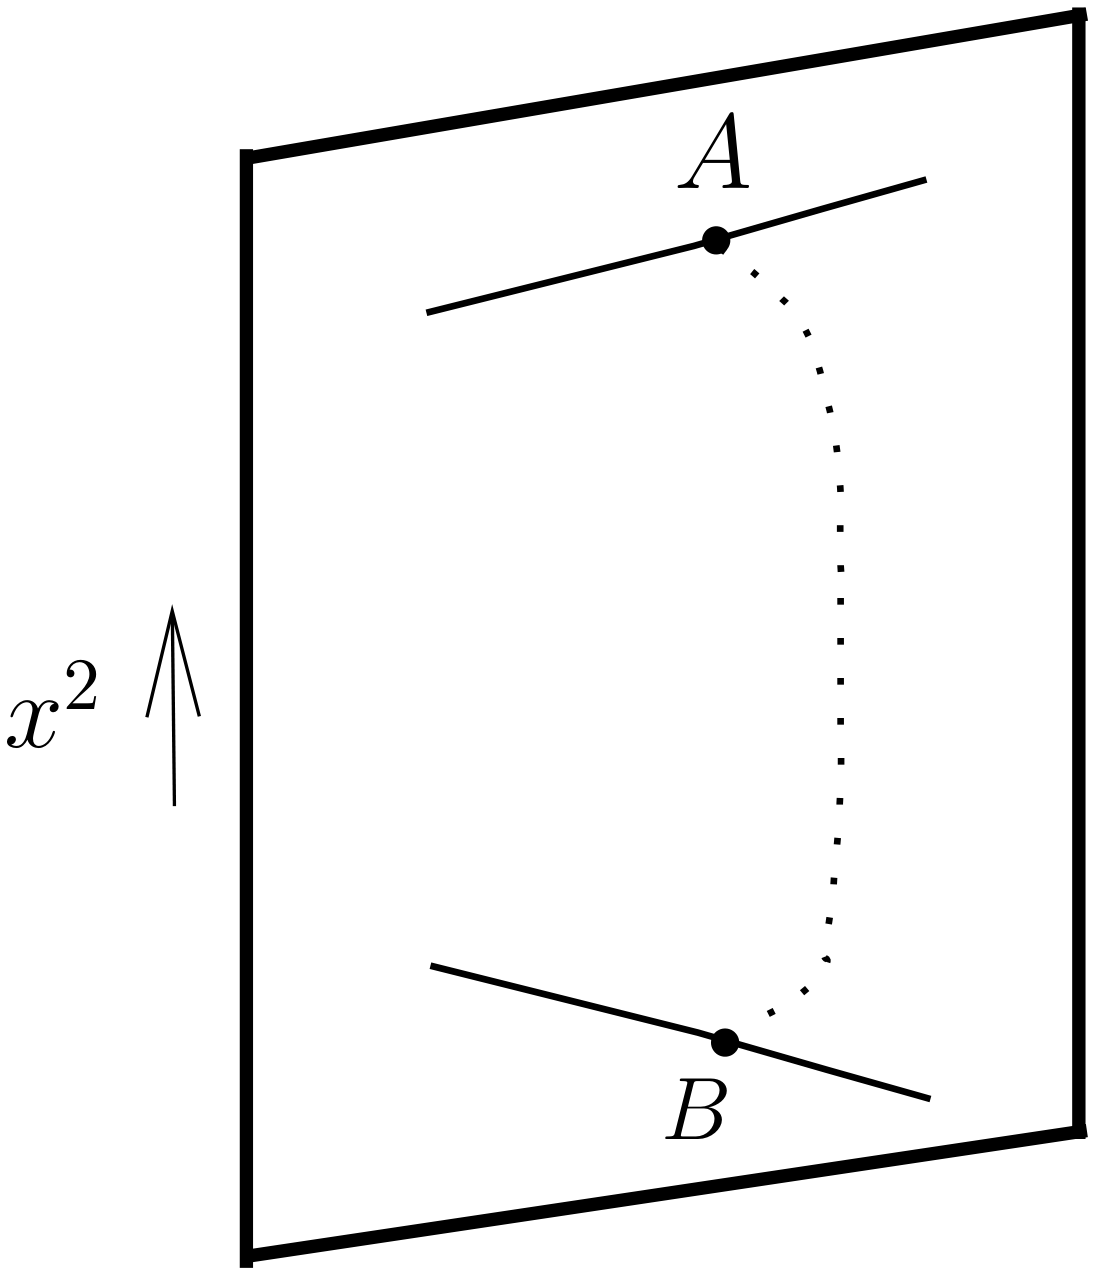
\includegraphics[width=3in]{figs/Fig25.png}
 \end{center}
\caption{\small 图~\ref{soliton} 所述荷交换过程的另一种视图，用以展示 $y$ 方向的作用（此处该方向被画成垂直于包含两股的平面）。在 $x^2$ 方向上相距很远的两个边界点 $A$ 与 $B$ 之间传播的孤子，会弯离边界，以达到对应于裸 Miura oper 解的 $y$ 值。（原稿第 84 页）\label{bending}}
\end{figure}

我们已经对强对称性破缺下四维 BPS 方程的解获得了直观图像：它们描述在奇异磁单极子股之间拉展开的光滑磁单极子构型。每个构型对纽结不变量的贡献是两类因子的乘积。一类来自从微观非阿贝尔理论到阿贝尔理论的映射，另一类则在阿贝尔理论中计算。第一类因子出现在成对的股被产生或湮灭之处、以及光滑磁单极子被边界奇异磁单极子发射或吸收之处。在阿贝尔描述中，光滑磁单极子看起来也是荷为 $2$ 的奇异磁单极子，但并不附着于边界。整个构型看起来像一张磁单极子股构成的网，阿贝尔理论给它赋予一个整体的 $q$ 幂次。

\subsubsection{对偶 Chern-Simons 理论中的类比}\label{dualch}

把这一图像一路追溯到三维 Chern-Simons 理论——即在我们经由种种对偶到达本文所研究的四维描述之前——是件有趣的事。
联系这两幅图像的关键一步是 $S$-对偶；幸运的是，它在强对称性破缺下非常透明，因为它约化为阿贝尔规范场论中的电磁对偶。我们立刻得到对如下构型的求和：大质量 $W$-玻色子拉展在 Wilson 线之间，并且只携带朝正 $x^2$ 方向流动的电荷。

这提示我们在非阿贝尔 Chern-Simons 理论中寻找能产生这一效果的规范条件。它很容易被认出：可以选取一种“部分”轴规范固定，把规范场的 $A_2$ 分量约化到 Cartan 子代数中。我们把非阿贝尔规范场写成 $A=B\frak t_3+W_+\frak t_++W_-\frak t_-$，并对 $W_\pm$ 施加 $A_2=0$ 规范条件；此处不必为对角规范场 $B$ 作规范选择。带电 $W$-玻色子的作用量于是约化为
\begin{equation}
\frac{\k^\vee}{4\pi}\int \d^3x \,\,W_+ D_2 W_-,~~~   D_2=\frac{\partial}{\partial x^2}+[B_2,\,\,\cdot\,\,].
\end{equation}
传播子的方程为
\begin{equation}
D_2 G(x,y) = \frac{2\pi}{\k^\vee}\delta^3(x-y)
\end{equation}
其解为
\begin{equation}\label{dox}
\frac{2\pi}{\k^\vee} 
\exp\left(\int_{x^2}^{y^2} B_2\right)\, \delta(x^1-y^1) \delta(x^3-y^3) \theta(x^2 - y^2),
\end{equation}
后者只描述荷朝正 $x^2$ 方向的传播。
相当清楚的是，这样的部分规范固定会给出顶点模型的某个版本，尽管精确计算顶点权重可能颇为棘手。所需的计算大概与在通常轴规范下研究 Chern-Simons 理论（例如见文献~\cite{AS,Hahn}）、或在某种几乎轴规范下研究 Chern-Simons 理论（文献~\cite{Wetering}）时的计算有些类似。使用复化的轴规范来导出 Knizhnik-Zamolodchikov 方程（文献~\cite{FK}）也与此有些类似。

% [Tutor Note: 物理图像] $\theta(x^2-y^2)$ 阶跃函数是这一段的要点：它把传播严格限制在 $x^2$ 增大的方向，即“电荷只能朝正 $x^2$ 流动”。若没有它，传播子就是双向的，顶点模型里就会出现逆向的弦，从而无法得到只有一种流向的顶点权重。这与图~\ref{vertexweights} 中“正荷只能从底部流入”的规则是同一件事的场论表述。

\subsection{上至六维}
着眼未来的范畴化（categorification），把这一阿贝尔图像一路提升到六维是有用的。毕竟，在存在强对称性破缺时，六维 $(0,2)$ 理论并不那么神秘。它是自对偶二形式与重的大质量动力学 BPS 弦耦合的理论。
导致纽结不变量的六维框架，涉及乘积 $\R \times M_3 \times D$ 上的六维理论，其中 $D$ 是一个几何上半无限雪茄的 $\R^2$（见式 (\ref{cigarl})）。纽结本身由置于雪茄尖端的打结二维缺陷表示。$q$-分次来自 $D$ 的旋转对称性所导出的守恒角动量。

在不存在对称性破缺时，$D$ 上的度规是雪茄型的而非欧几里得度规，这一点对于得到良定义的缺陷态空间很重要。置于平坦六维空间中的缺陷会与体 SCFT 强耦合。另一方面，在存在对称性破缺时，红外物理是自由的，我们可以希望从动力学重弦与缺陷的束缚态中恢复态空间。此时雪茄几何将不起重要作用，$D$ 可以换成一个平坦的 $\R^2$。

现在，我们专门取 $M_3 = \R^3$，并且为简洁起见取纽结与时间无关。
不含时的动力学弦的 BPS 条件非常简单：它必须是直的，并与对称性破缺方向（我们仍取为 $x^2$ 方向）对齐。这实际上就是光滑磁单极子所满足条件的六维提升，并且投影到 $x^2$ 上时给出相同的顶点模型图像。在阿贝尔低能描述中，缺陷股有两个可能的基态，它们具有相反的二形式荷。与动力学弦的汇合允许二形式荷发生跳跃。

有趣的问题是，从六维的角度重现顶点模型的权重。这既包括由弦作为源的自对偶二形式阿贝尔理论的贡献，也包括弦的世界体积理论的贡献。我们在此不计算前者，但可以对后者给出一些洞见。

如图~\ref{vertexweights} 所总结的，对 Jones 多项式有贡献的荷交换过程的顶点模型权重为
\begin{equation}
\label{twof}q^{\pm 1/4}-q^{\mp 3/4}. \end{equation}
  在六维图像中，Jones 多项式应当来自对 BPS 态求和，权重为 $q^P(-1)^F$，其中 $P$ 是与 $D$ 的旋转相对应的守恒荷，而 $F$（可以宽松地称为费米子数）是某个 $R$-对称生成元。
我们把 (\ref{twof}) 中两项之间的相对因子 $-q^{\pm 1}$ 解释为：连接纽结中两股的 BPS 弦有两个物理态，它们在角动量上相差 1（以解释因子 $q^{\pm 1}$）、在费米子数上也相差 1（以解释负号）。
为理解这一点，我们可以把注意力集中在那两条交叉的股以及拉展在它们之间的弦上。关键在于：单股是半 BPS 的，两条不平行的股是四分之一 BPS 的，但两股交换一条 BPS 弦的构型把对称性进一步破缺到八分之一 BPS。因此该弦破缺两个超荷，从而必须有两个基态，它们被破缺超荷的作用互换。这立刻给出所需的量子数差。

% [Tutor Note: 物理图像] “破缺两个超荷 ⇒ 两个基态”的推理是本节最容易被跳过的环节：两个实超荷合成一个复的费米型升降算符 $Q$，其作用在真空上给出一个二重简并（$|0\rangle$ 与 $Q|0\rangle$），故基态数为 2；这也正是超荷多重态维数的一般规律。若破缺的超荷数为 $2n$，基态简并度应为 $2^n$，本文情形 $n=1$。这一简并度的“量子数差”（角动量差 1、费米子数差 1）正是顶点权重中 $-q^{\pm 1}$ 相对因子的来源。

因此，系统的近似基态空间可以如下描述。设 $\mathcal S$ 为顶点模型的构型集合（用 $+$ 或 $-$ 标记各股，并在标号发生跳跃的交叉处接上光滑弦）。对每条光滑弦，引入一个二维 Hilbert 空间，其量子数由上一段推出。对每个 $s\in \mathcal S$，引入一个 Hilbert 空间 $\mathcal H_s$，它定义为与各光滑弦相伴的二维因子的张量积。于是 BPS 态空间的一个近似 $\mathcal H_0$ 为 $\mathcal H_0=\oplus_{s\in\mathcal S}\mathcal H_s$。
$\mathcal H_0$ 的分次（按角动量与费米子数）受到由弦系统作为源的阿贝尔场构型的影响；例如，自对偶阿贝尔张量场可以携带角动量。

为计算 Khovanov 同调，需要求出作用在这个近似基态空间上的微分，其办法是寻找在不同态之间（在过去与未来之间）插值的瞬子构型。
含时 BPS 弦的 BPS 条件仍然相当透明。其世界面应当在复坐标 $x^0 + i x^2$ 与 $x^1 + i x^3$ 下全纯。注意：沿 $x^2$ 方向拉展的不含时弦（因而由 $x^0$ 与 $x^2$ 参数化，$x^1$ 与 $x^3$ 固定）确实具有全纯的世界体积。

因此我们预期能够由 $\R \times M_3$ 中终止于纽结的全纯曲线的数据来构造 Khovanov 同调的微分。这一途径看来对未来的发展颇有前景。
